\chapter{PID controller design}

\section{Specifying the problem}
There are 2 simple approaches in designing a controller: active (PD design then PI design) or passive (lead compensator design then lag compensator design), which are referred to as PID and lag-lead compensator. In this modeling project, the active controller PID is used. The design technique consists of the following steps:
\begin{enumerate}
	\item Evaluate the performance of the uncompensated system to determine how much improvement in transient response is required.
	\item Design the PD controller to meet the transient response specifications. The design includes the zero location and the loop gain.
	\item Simulate the system to be sure all requirements have been met.
	\item Redesign if the simulation shows that requirements have not been met.
	\item Design the PI controller to yield the required steady-state error.
	\item Determine the gains, $ K_p $, $ K_i $ and $ K_d $.
	\item Simulate the system to be sure all requirements have been met.
	\item Redesign if simulation shows that requirements have not been met.
\end{enumerate}

Combining all design problems from previous chapters, the design requirements for PID controller is

\textbf{Design a PID controller so that the system can operate with a 2 fold improvement in settling time at $ 10\% $ overshoot and zero steady-state error for a ramp input.}

\section{Ideal derivative (PD) controller}
Following the guidelines above, the ideal derivative controller is designed first. Using the calculated result, the uncompensated closed-loop poles are $ s = -2.5\pm j3.411 $ with a gain $ K=0.9827 $. The settling time must be a half of the uncompensated one. Therefore,
\begin{equation}
	T_s = \dfrac{4}{\zeta \omega_n} = \dfrac{4}{0.591 \omega_n} = 1.6/2 \Rightarrow \omega_n = 8.46
\end{equation}

The real part of the compensated pole is:
\begin{equation}
	\sigma_d = -\zeta\omega_n = -0.591\times 8.46 = -5
\end{equation}

The imaginary part of the compensated pole is:
\begin{equation}
	\omega_d = \omega_n\sqrt{1-\zeta^2} = 8.46\sqrt{1-0.591^2} = 6.824
\end{equation}

Therefore, the desired compensated closed-loop pole are $ s = -5\pm j6.824 $. Assume that the compensator zero is located at $ -z_c $ and the value $ s = -5 + j6.824 $, the total angle is
\[
\begin{array}{ll}
\theta & = \angle (s+z_c) - \angle (s+0) - \angle (s+5)\\
&  = \angle (-5 + j6.824 + z_c) - 126.23^\circ - 90^\circ = -180^\circ\\
&\Leftrightarrow \angle (-5 + j6.824 + z_c) = 36.23^\circ\\
&\Leftrightarrow \dfrac{6.824}{-5 + z_c} = \tan 36.23^\circ\\
&\Leftrightarrow z_c = 14.31
\end{array}
\]

Thus, the PD controller is $ G_{PD} = s+14.31 $. With the new zero introduced to the open-loop transfer function, another gain $ K $ must be found such that the damping ratio $ \zeta = 0.591 $ intersects the root locus of equation $ K(s+14.31)\frac{18.2}{s(s+5)} $. The corresponding gain $ K $ is

\begin{equation}
	\begin{array}{ll}
	K &= \dfrac{1}{|s+14.31|}\dfrac{|s||s+5|}{18.2}\\
	&= \dfrac{1}{|-5 + j6.824+14.31|}\dfrac{|-5 + j6.824||-5 + j6.824+5|}{18.2}\\
	&= 0.042
	\end{array}
\end{equation}
Thus, the transfer function of PD controller is
\begin{equation}
	G_{PD} = K(s+14.31) = 0.042s + 0.6
\end{equation}

\section{Ideal integral (PI) controller}
The PI controller reduces the steady-state error of ramp input $ e_{ramp}(\infty) $ to 0. Arbitrarily choose the zero $ z_c = -0.1 $ so that the controller does not significantly affect the transient response of the PD compensated system. Thus, the transfer function is
\begin{equation}
	G_{PI} = K\dfrac{s+0.1}{s}
\end{equation}

Using the root locus program, $ s = -4.422 \pm j6.034 $ is selected. Comparison is necessary to see if the gain $ K $ is closed to the previous value $ K_p = 0.9827 $. Using $ s = -4.422 + j6.034  $ as the value for calculation, the angle is
\[
\begin{array}{ll}
\theta & = \angle (s+14.31) + \angle (s+0.1) - 2[\angle (s+0)] - \angle (s+5)\\
& = \angle (-4.422 + j6.034 + 14.31) + \angle (-4.422 + j6.034+0.1) \\
& \qquad - 2[\angle (-4.422 + j6.034+0)] - \angle (-4.422 + j6.034+5)\\
& = 31.393^\circ + 125.613^\circ - 2\times 126.236^\circ - 84.528^\circ\\
& = -179.994^\circ \approx -180^\circ \\
\end{array}
\]
which is near the root locus but does not significantly affect the transient response. The corresponding gain $ K $ is
\[
\begin{array}{ll}
K &= \dfrac{|s|}{|s+0.1|}\dfrac{|s||s+5|}{18.2|s+14.31|}\\
&= \dfrac{|-4.422 + j6.034|}{|-4.422 + j6.034+0.1|}\dfrac{|-4.422 + j6.034||-4.422 + j6.034+5|}{18.2|-4.422 + j6.034+14.31|}\\
&= 0.217
\end{array}
\]

In summary, the transfer function of the PID controller is
\begin{equation}
	G_{PID} = 0.217\dfrac{(s+0.1)(s+14.31)}{s} = 0.217s + 3.127 + \dfrac{0.31}{s}
\end{equation}
with $ K_p = 3.127 $, $ K_i = 0.31 $ and $ K_d = 0.217 $.

\section{Graphic results}
\subsection{Compensated pole of the PD controller $ z_c $}
\begin{minted}{python}
	from control import *
	from numpy import *
	from matplotlib.pyplot import *
	import sympy as sp
	
		
	G = tf([18.2], [1,5,0])
	rlocus(G)
	
	zeta = -log(0.1) / sqrt(pi**2 + log(0.1)**2)
	x = array([-10,0])
	
	plot(x,tan(pi-arccos(zeta))*x)
	
	Ts = 1.6/2
	omg_n = 4/Ts/zeta
	sig_d = -zeta*omg_n
	omg_d = omg_n*sqrt(1-zeta**2)
	s_d = sig_d + 1j*omg_d
	
	z_c = sp.symbols('z_c')
	f = omg_d/(sig_d+z_c) - tan(angle(s_d+0) + angle(s_d+5) - pi)
	z_c = sp.solve(f)
	print(z_c)
\end{minted}

\begin{figure}[ht]
	\centering
	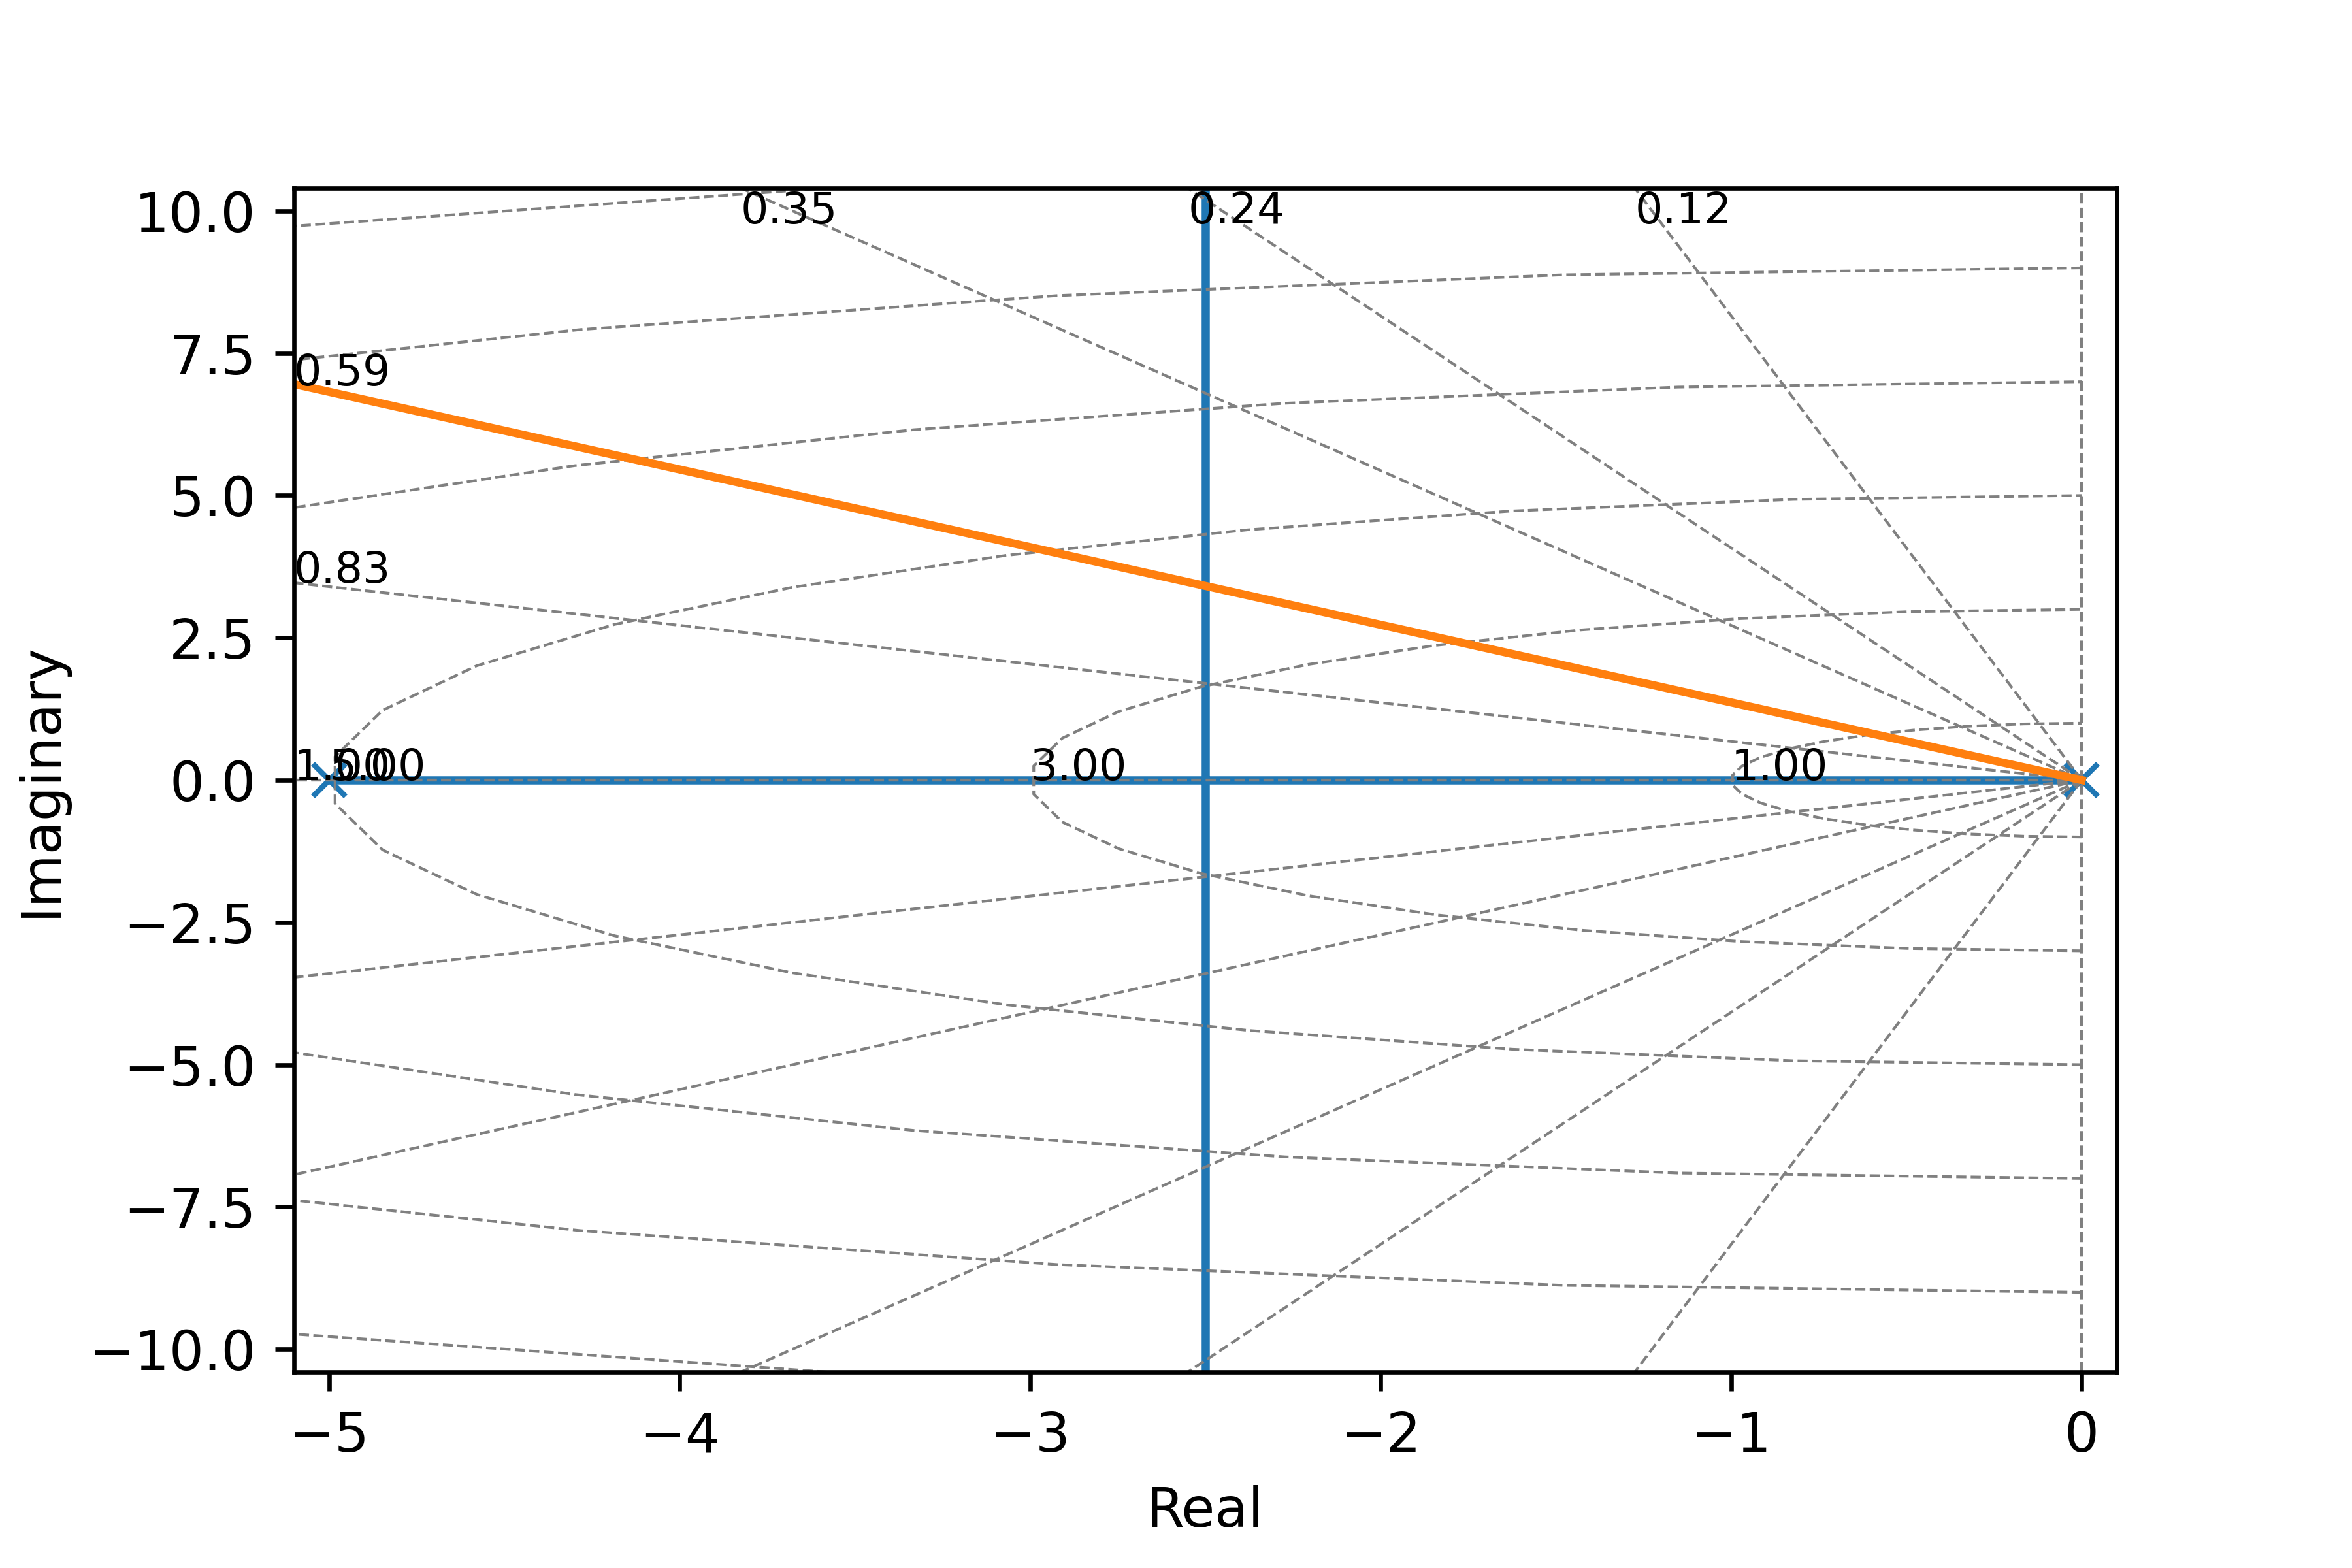
\includegraphics[width=0.7\linewidth]{rlocus_PD}
	\caption{Root locus of the open-loop uncompensated system}
\end{figure}

\subsection{Transfer function of the PID controller}
\begin{minted}{python}
	from control import *
	from numpy import *
	from matplotlib.pyplot import *


	s = tf('s')
	G = tf([18.2],[1,5,0]) * (s+14.31) * (1+0.1/s)
	rlocus(G)
	
	zeta = -log(0.1) / sqrt(pi**2 + log(0.1)**2)
	x = array([-10,0])
	
	plot(x, tan(pi-arccos(zeta))*x)
	print(0.217*poly([-0.1,-14.31]))
\end{minted}

\begin{figure}[ht]
	\centering
	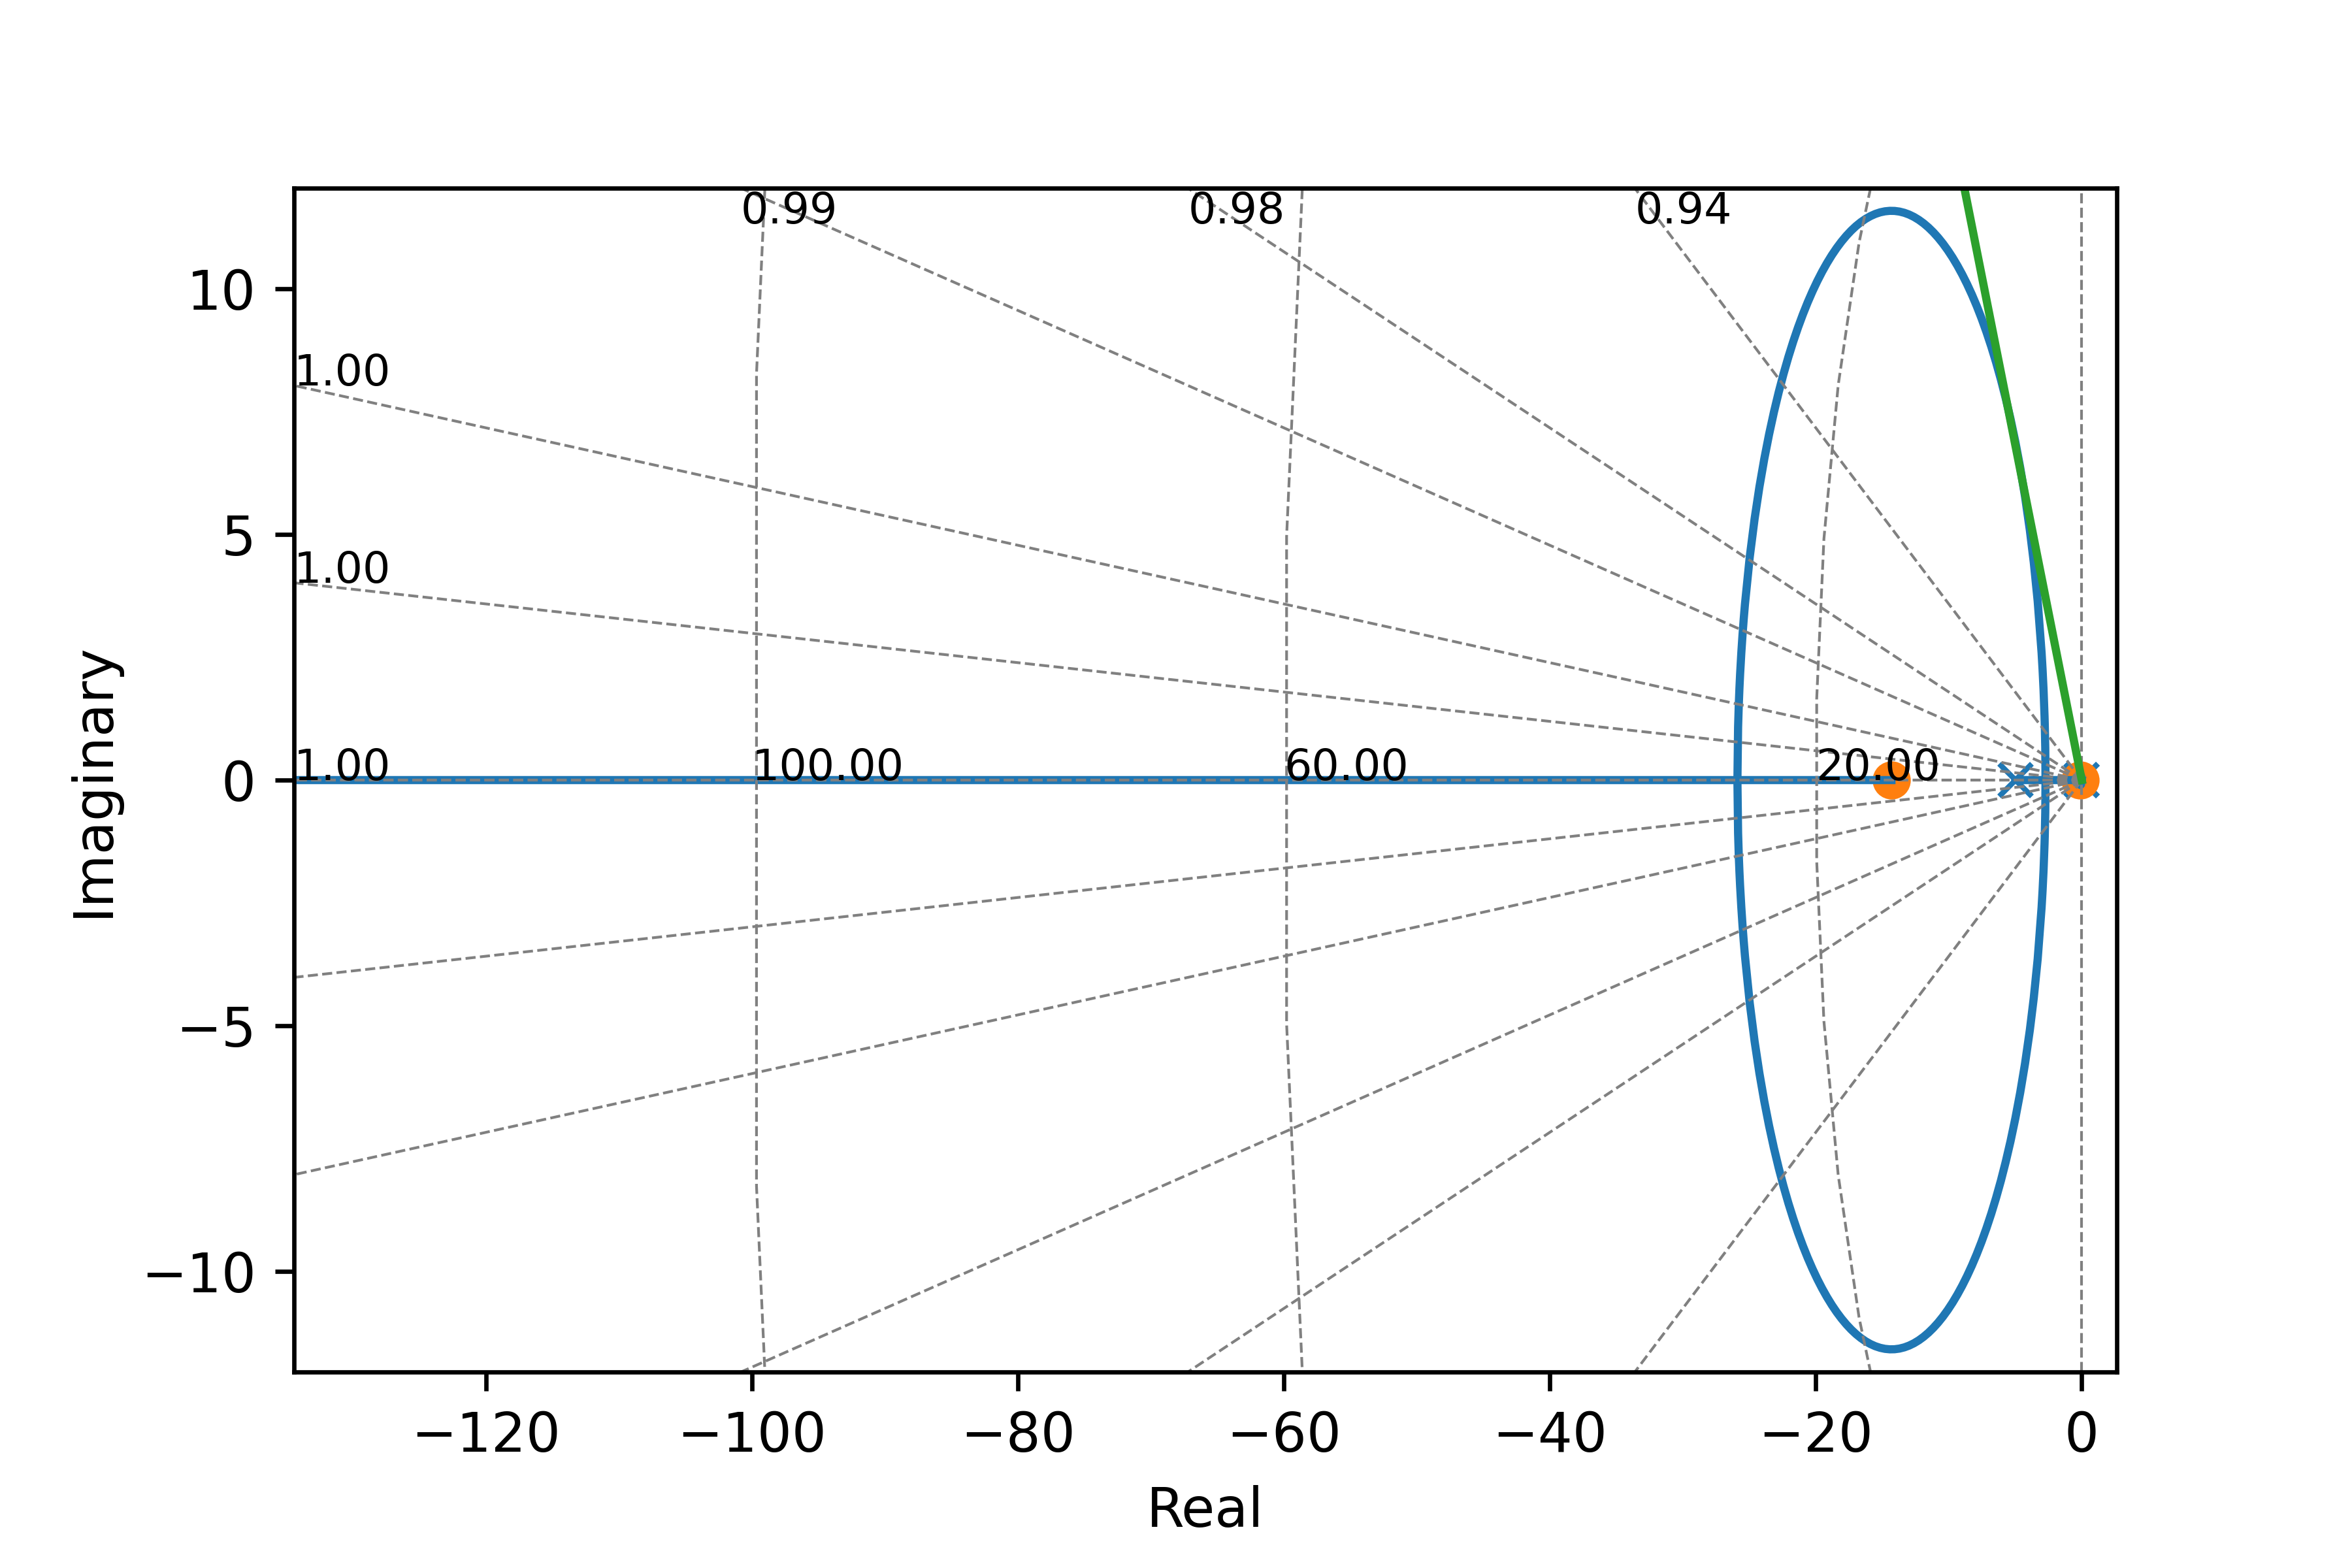
\includegraphics[width=0.7\linewidth]{rlocus_Kpi2}
	\caption{Root locus of the open-loop PD compensated system}
\end{figure}

\subsection{Transient response of the system}
\subsubsection{Step response}
\begin{minted}{python}
	from control import *
	from numpy import *
	from matplotlib.pyplot import *
	
	
	s = tf('s')
	G = tf([18.2],[1,5,0]) * (s+14.31) * (1+0.1/s)
	sys = feedback(0.217*G, 1)
	
	T = linspace(0, 3, 1000)
	
	plot(*step_response(sys, T=T))
\end{minted}

\begin{figure}[ht]
	\centering
	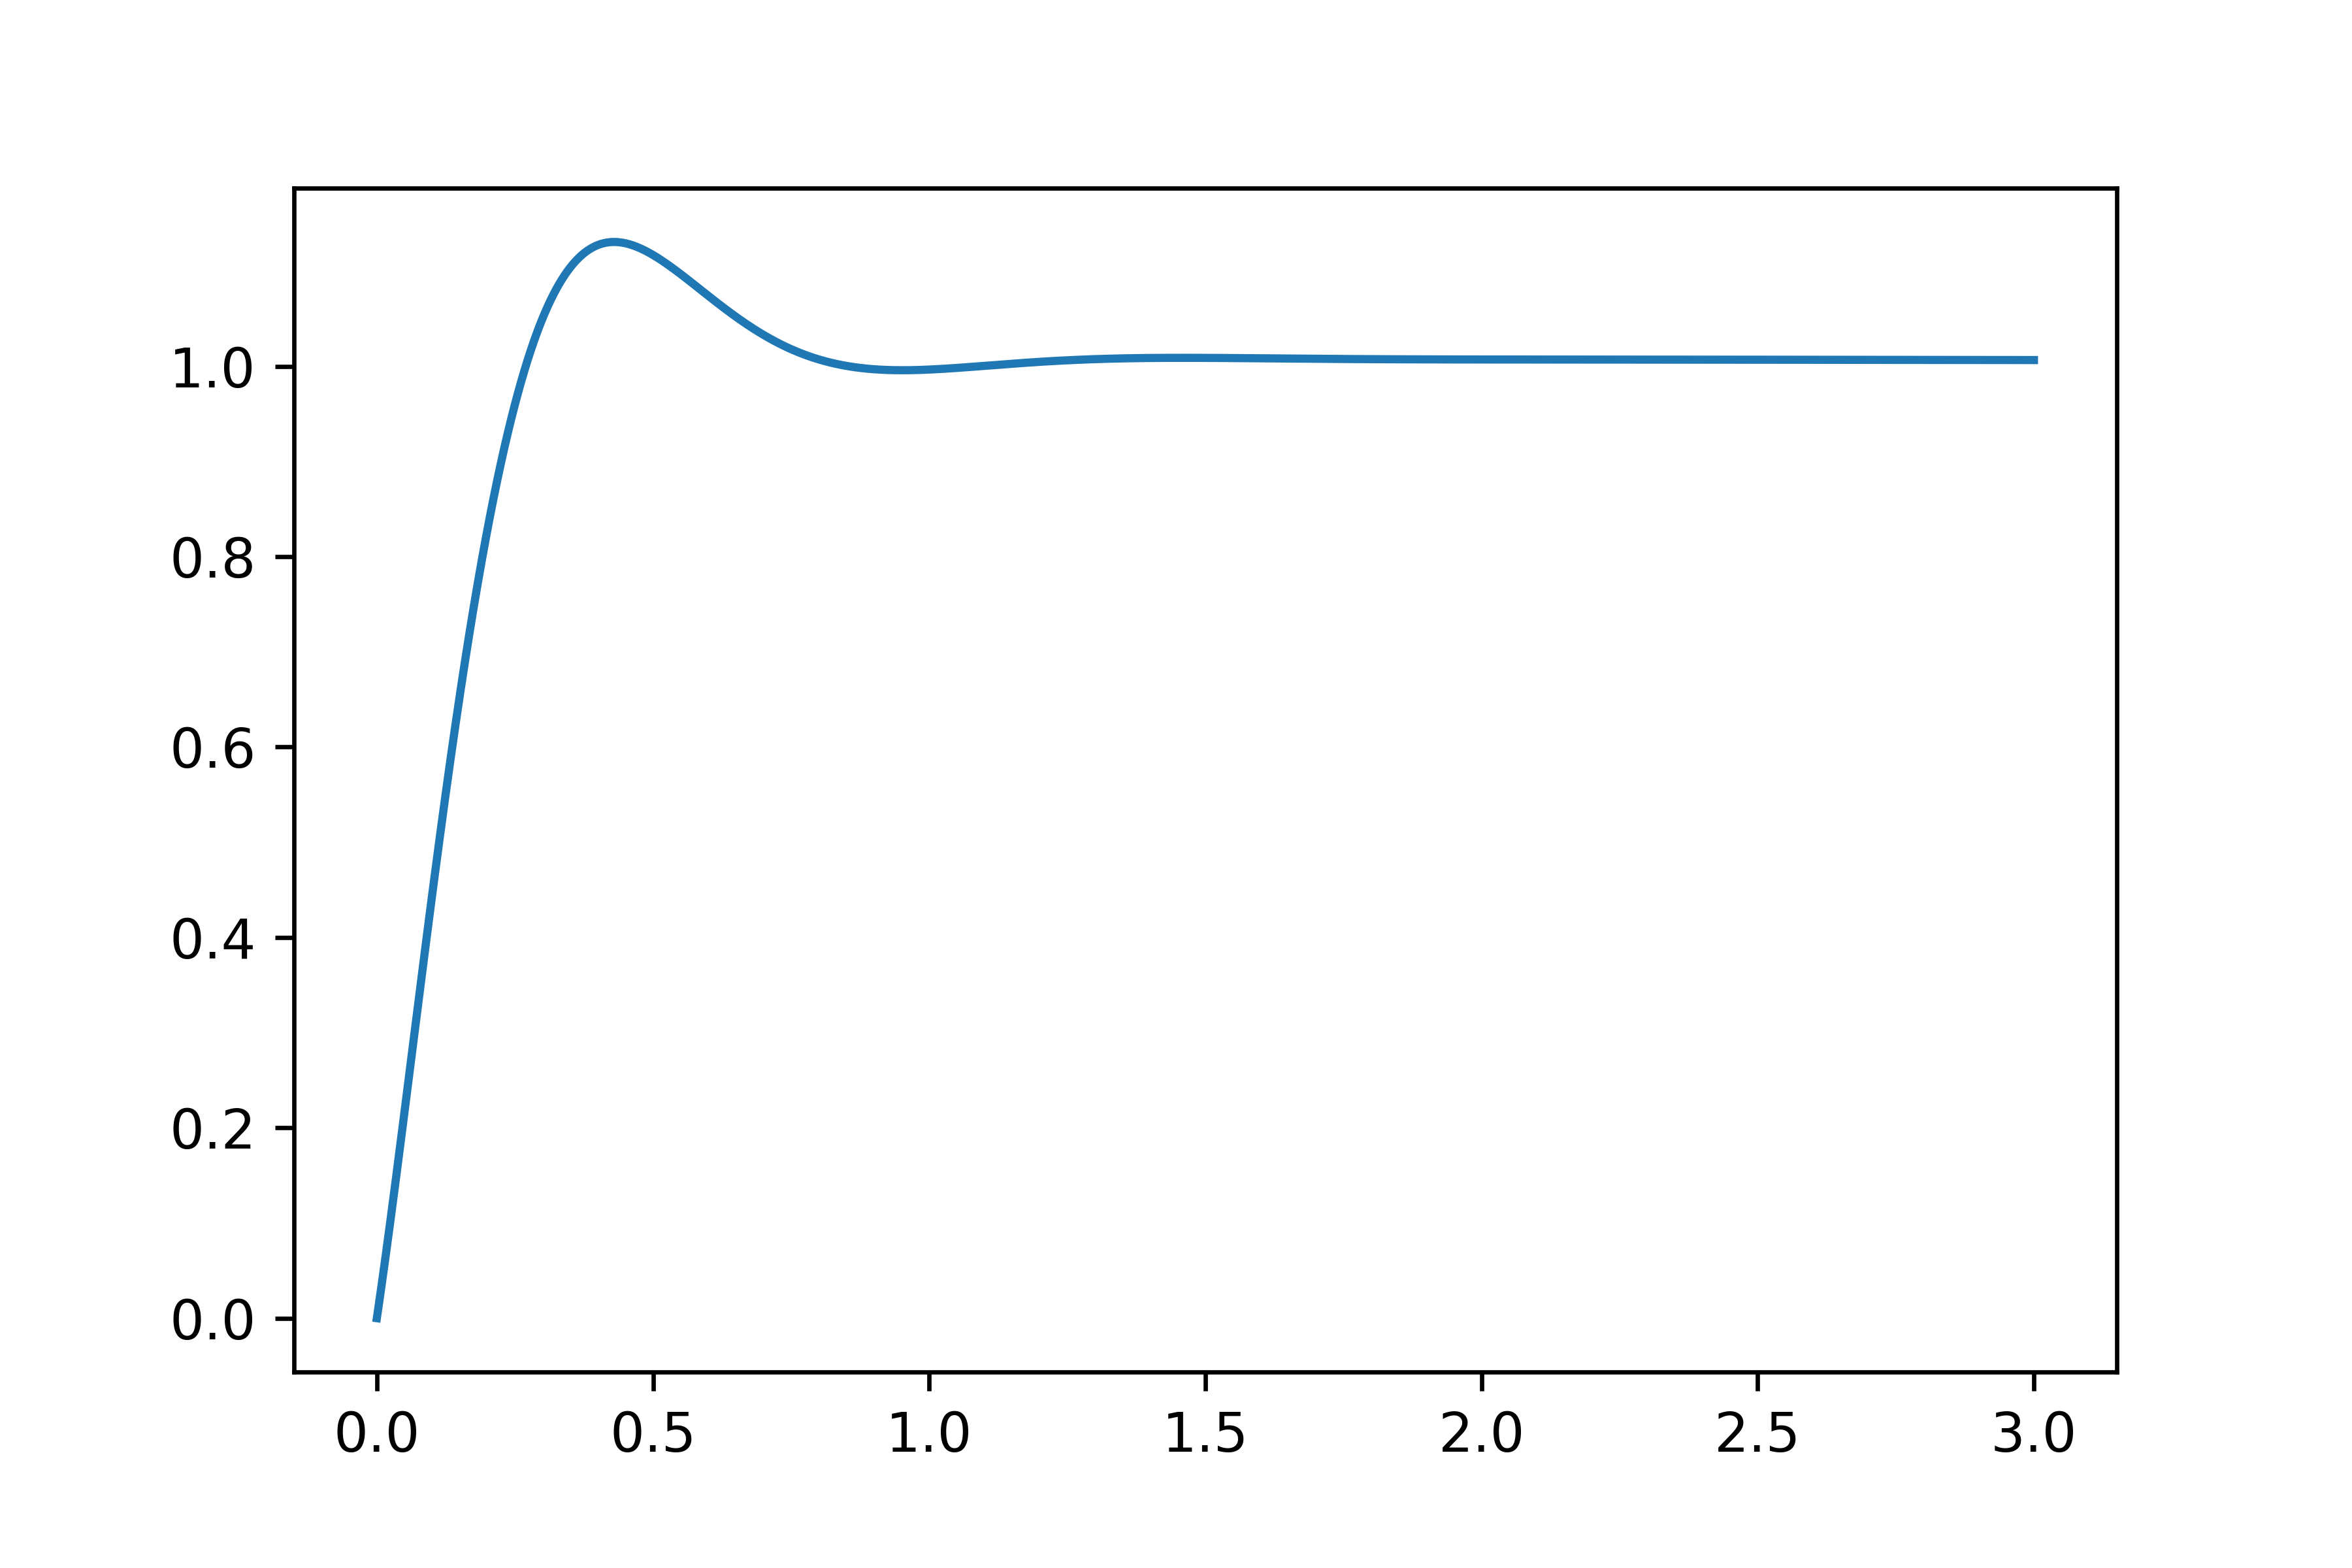
\includegraphics[width=0.7\linewidth]{step_pid}
	\caption{Step response of the system using PID controller}
\end{figure}

\subsubsection{Ramp response}
\begin{minted}{python}
	from control import *
	from numpy import *
	from matplotlib.pyplot import *
	
	
	s = tf('s')
	G = tf([18.2],[1,5,0]) * (s+14.31) * (1+0.1/s)
	sys = feedback(0.217*G, 1)
	
	U = T = linspace(0, 0.8, 1000)
	yout, T, xout = lsim(sys, U, T)
	
	plot(T, U, color='gray', label='ramp input')
	plot(T, yout, color='blue', label='ramp response')
	legend()
\end{minted}

\begin{figure}[ht]
	\centering
	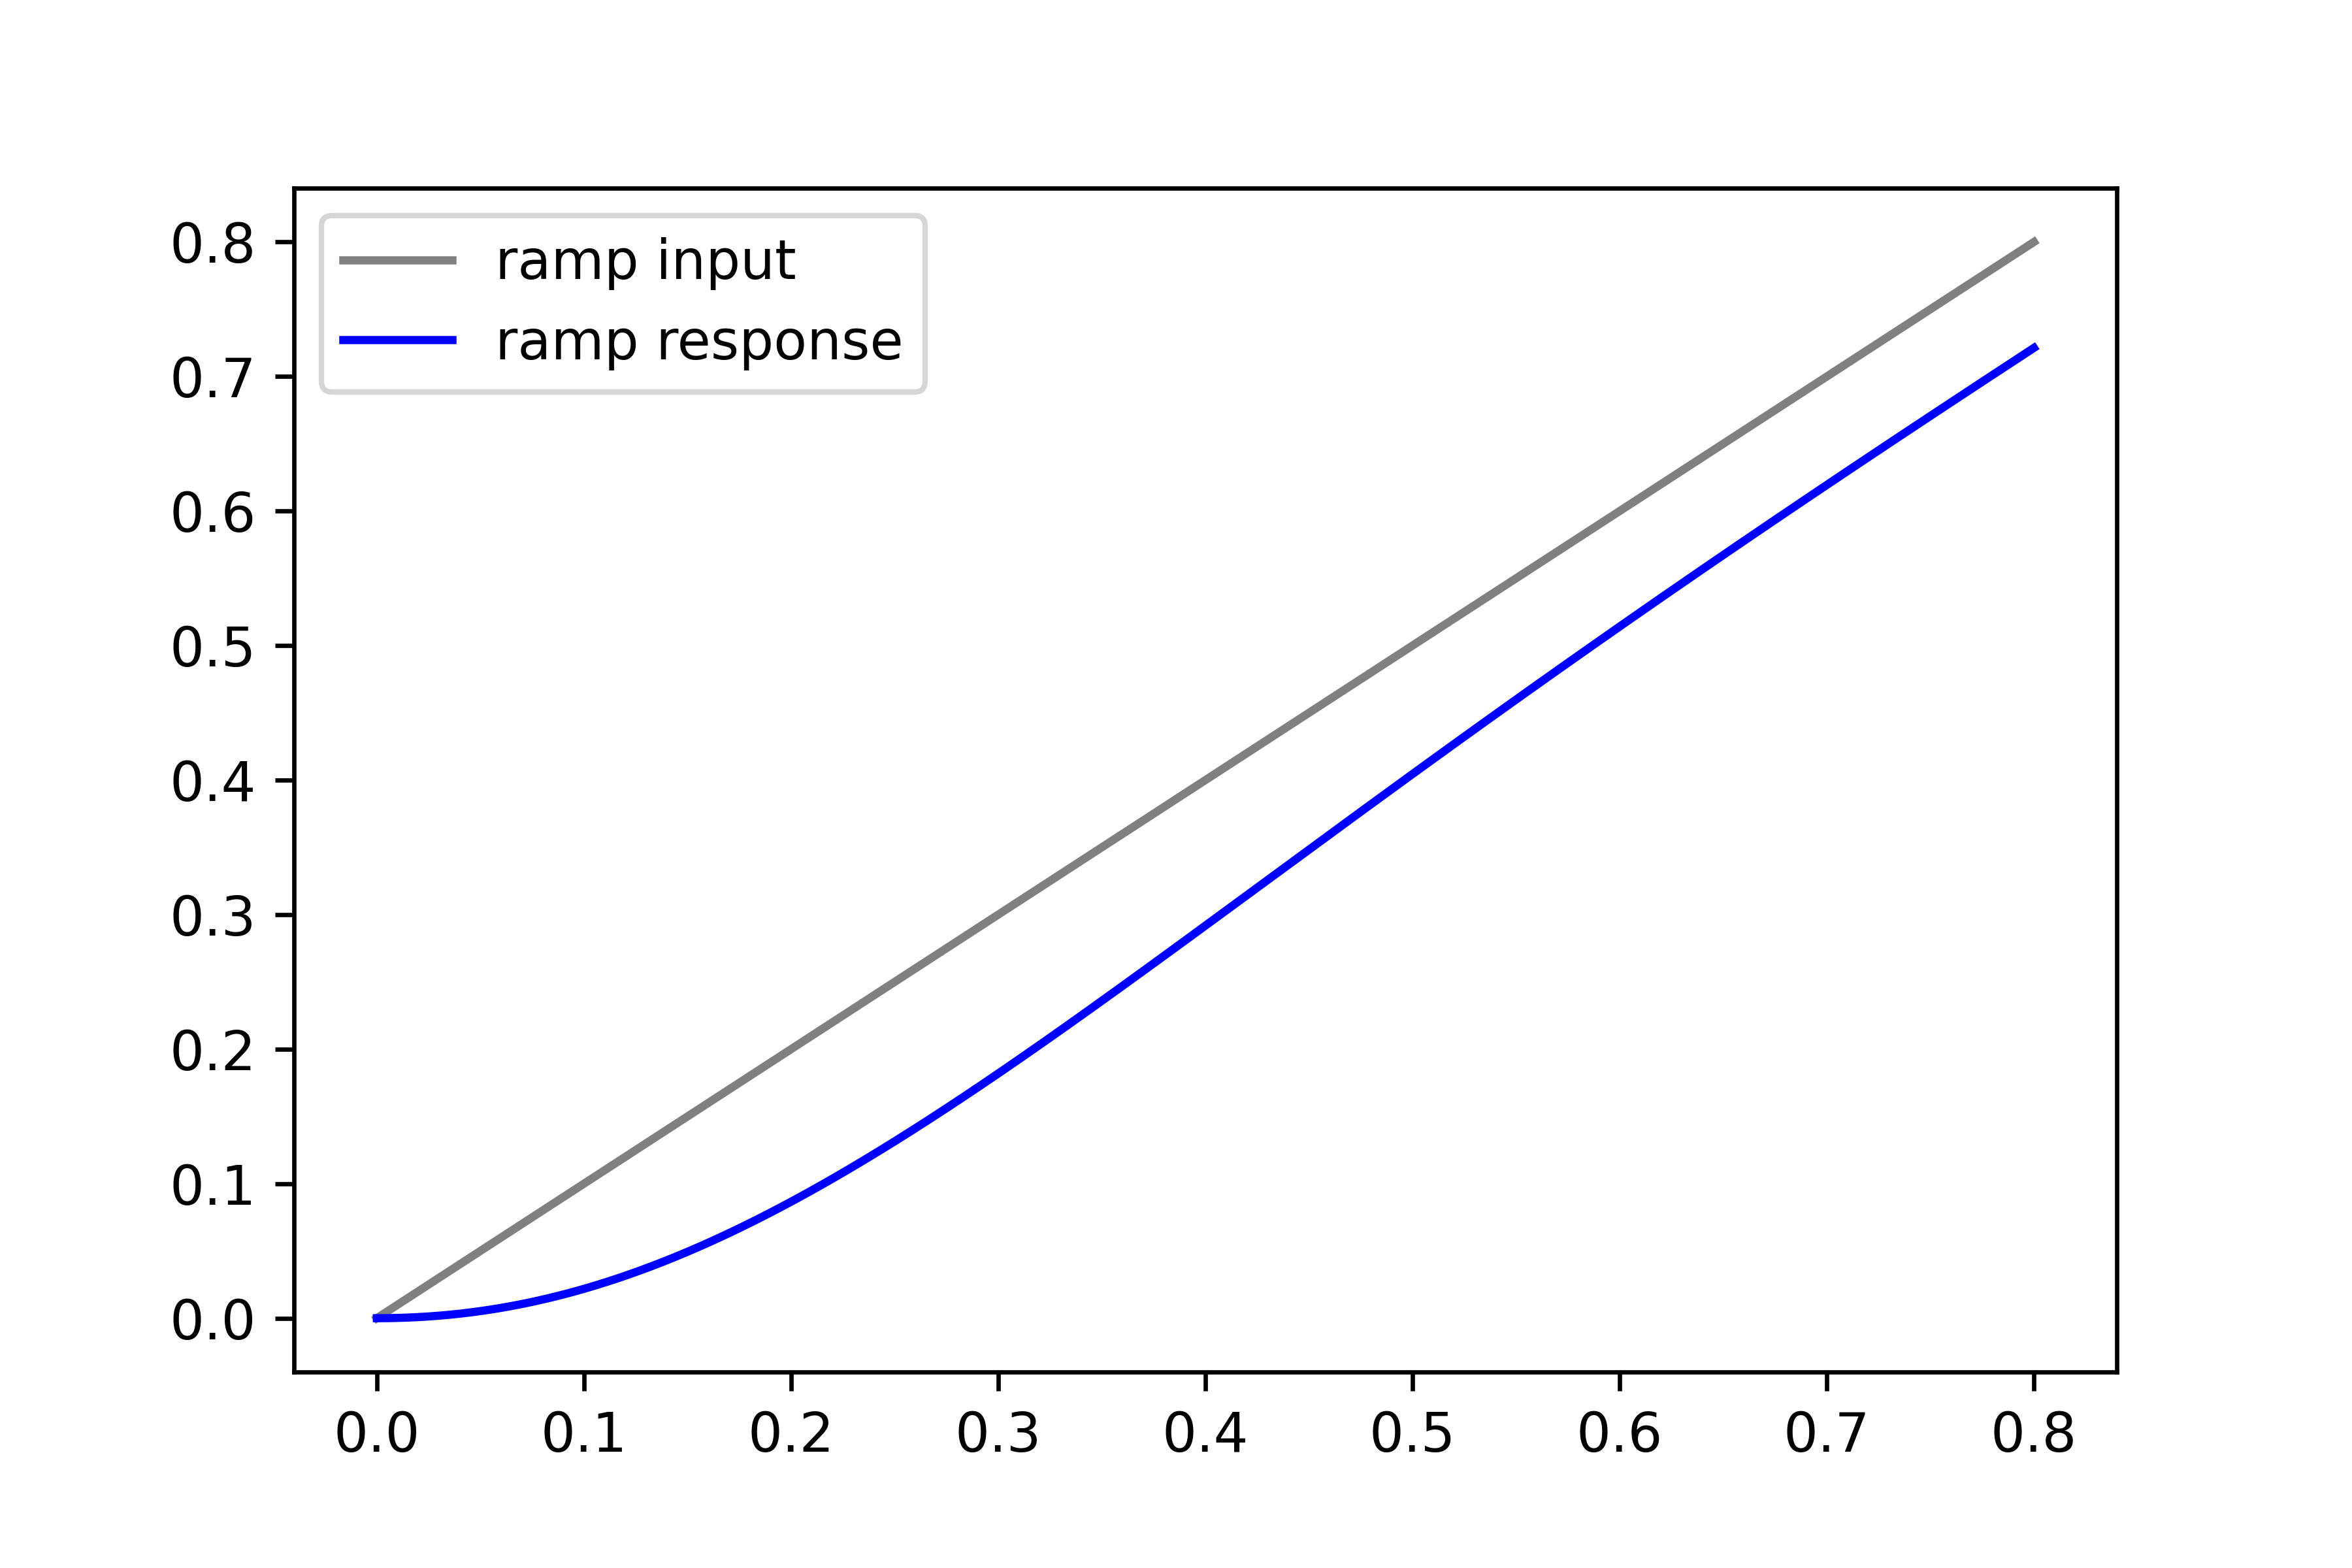
\includegraphics[width=0.7\linewidth]{ramp_pid}
	\caption{Ramp response of the system using PID controller}
\end{figure}